\begin{flushright}
    \begin{figure}[H]
        \centering
        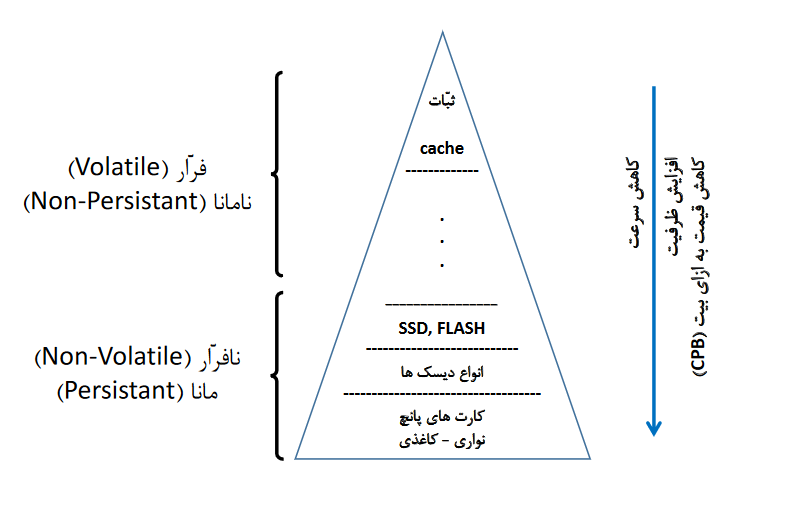
\includegraphics[width=0.7\textwidth]{source/memory-hierarchy}
        \caption{سلسه مراتب حافظه}
        \label{fig:memory-hierarchy}
    \end{figure}

    به نکات زیر با توجه به تصویر سلسله مراتب حافظه دقت کنید.
    \begin{itemize}
        \item باحرکت از سمت بالا به پایین هرم:
        \begin{enumerate}
            \item سرعت دسترسی به حافظه کمتر می‌شود.
            \item حجم حافظه بیشتر می‌شود.
            \item قیمت به ازای هر بیت کاهش می‌یابد.
        \end{enumerate}
        \item حافظه‌های قسمت بالا هرم معمولا فرار هستند و با خاموشی سامانه و جریان نداشتن برق، اطلاعات خود را از دست می‌دهند.
        \item برای ذخیره‌سازی اطلاعات نوعا از حافظه‌های نافرار که در قسمت پایین‌تر هرم قرار دارند استفاده می‌شود.
    \end{itemize}

    \subsubject{HDD}{files/sub-memory-hierarchy/HDD}
    \subsubject{نگاه انتزاعی به حافظه}{files/sub-memory-hierarchy/abstract-view}

\end{flushright}